% 2008 年天津卷理科第 14 题：平行四边形 ABCD，对角线 AC、BD 已给出向量坐标。
% 来源 PDF：gaokaomath-src/普通高考/2008/2008天津理.pdf
% SHA-256：e2442be3c0179c888e74b31dda58e749b6ab84ac8cccf86eae4677ab3843f48b
% 原页：2008天津理.pdf 第 1 页（A3 三栏）第 2 栏，书页码 487。
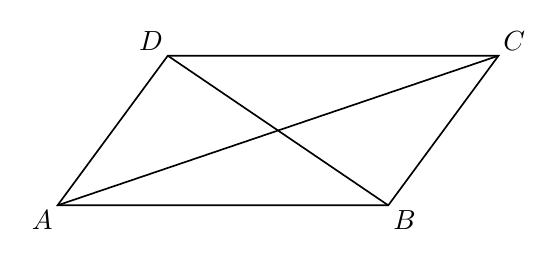
\begin{tikzpicture}[scale=1.0, semithick,
  every node/.style={inner sep=1.5pt}]
  \coordinate (A) at (0,0);
  \coordinate (B) at (4.2,0);
  \coordinate (C) at (5.6,1.9);
  \coordinate (D) at (1.4,1.9);

  \draw (A) -- (B) -- (C) -- (D) -- cycle;
  \draw (A) -- (C);
  \draw (B) -- (D);

  \node[below left] at (A) {$A$};
  \node[below right] at (B) {$B$};
  \node[above right] at (C) {$C$};
  \node[above left] at (D) {$D$};
\end{tikzpicture}
